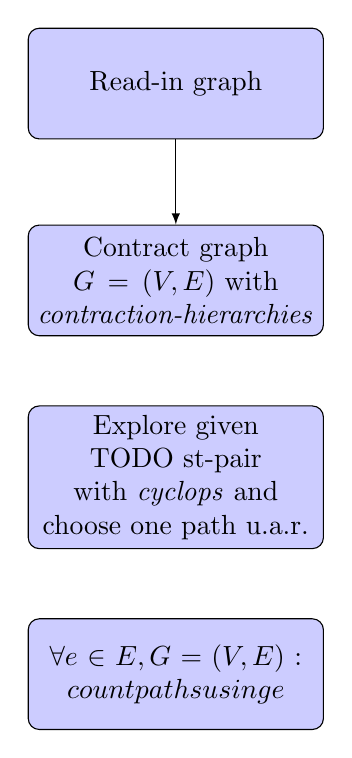
\begin{tikzpicture}[auto, rounded corners=0, node distance = 3cm, x=1cm, y=1cm] {%
    % style

    % draw
    % Draw borders

    % text badly centered
    % better use 'align=flush center'

    \tikzstyle{decision} = [%
        diamond,
        draw,
        fill = blue!20,
        text width = 4.5em,
        align = flush center,
        node distance = 3cm,
        inner sep = 0pt
    ]
    \tikzstyle{block} = [%
        rectangle,
        draw,
        fill = blue!20,
        text width = 10em,
        text centered,
        rounded corners,
        node distance = 2.5cm,
        minimum height = 4em
    ]
    \tikzstyle{cloud} = [%
        draw,
        ellipse,
        fill = red!20,
        node distance = 3cm,
        minimum height = 2em
    ]

    % arrow-styles
    % https://tex.stackexchange.com/questions/5461/is-it-possible-to-change-the-size-of-an-arrowhead-in-tikz-pgf
    \tikzstyle{line} = [draw, -latex]

    % Place nodes

    \node [block] (read-in_graph) {Read-in graph};
    \node [block, below of = read-in_graph] (contract_graph) {Contract graph $G=(V,E)$ with \textit{contraction-hierarchies}};
    \node [block, below of = contract_graph] (exploration) {Explore given TODO st-pair with \textit{cyclops} and choose one path u.a.r.};
    \node [block, below of = exploration] (analyzation) {$\forall e \in E, G = (V, E): count paths using e$};

    % Draw lines

    \path [line] (read-in_graph) -- (contract_graph);

    % \node [block] (init) {initialize model};
    % \node [cloud, left of=init] (expert) {expert};
    % \node [cloud, right of=init] (system) {system};

    % \node [block, below of=init] (identify) {identify candidate models};

    % \node [block, below of=identify] (evaluate) {evaluate candidate models};
    % \node [block, left of=evaluate, node distance=3cm] (update) {update model};

    % \node [decision, below of=evaluate] (decide) {is best candidate better?};

    % \node [block, below of=decide, node distance=3cm] (stop) {stop};

    % % Draw edges

    % \path [line] (init) -- (identify);
    % \path [line] (identify) -- (evaluate);
    % \path [line] (evaluate) -- (decide);
    % \path [line] (decide) -- node {no} (stop);

    % \path [line] (update) |- (identify);
    % \path [line] (decide) -| node [near start] {yes} (update);

    % \path [line,dashed] (expert) -- (init);
    % \path [line,dashed] (system) -- (init);
    % \path [line,dashed] (system) |- (evaluate);
} \end{tikzpicture}